\section{Assemblies of DC1 and Tsth20}
\label{section:assemblies}

For general assembly metrics of DC1 and Tsth20, the
QUAST\cite{Gurevich2013} tool was used. Results from QUAST are shown
in Table~\ref{table:assemblies}, from which we can make several
observations. In DC1 and Tsth20, the total contig counts are an order
of magnitude smaller when compared to the other NCBI RefSeq
assemblies, indicating highly contiguous assemblies from
nextDenovo\cite{Hu2024} and nextPolish\cite{Hu2020}. This is likely
due to the use of Nanopore sequencing in the assemblies of DC1 and
Tsth20. The total assembled lengths of DC1 and Tsth20 are similar when
compared to RefSeq assemblies, ranging from 38Mb to 42Mb, except in
the case of \textit{T. reesei}, which is known to have a significantly
smaller genome length\cite{Kubicek2019}, at roughly 33Mb.

The largest contig size for each assembly varies greatly. DC1 and
Tsth20 have the largest contigs of all assemblies being considered,
which is again likely due to the inclusion of long-read sequencing
data in the assembly process. The N50 values for all assemblies are
above 1Mb, with DC1 and Tsth20 N50s being at minimum two times larger
than others assemblies. N50 lengths nearing chromosomal lengths
indicates that assemblies of DC1 and Tsth20 are better assembled than
the other \textit{Trichoderma} assemblies. While chromosome-scale
contigs are not the sole indicator of genome quality, it does provide
confidence in the quality of the input data and resulting
assemblies. In general, the assemblies of DC1 and Tsth20 are of
similar length to existing \textit{Trichoderma} assemblies and the
number of contigs reported match the number of `chromosome' scale
contigs reported in other work\cite{Kubicek2019}.

\begin{table}
  \begin{center}
    \begin{tabular}{|c|c|c|c|c|c|c|}
      \hline
      Strain & Total Contigs & Total Length & Largest Contig & GC\% & N50 & L50 \\ \hline
      DC1 & 8 & 38.6 Mb & 11.49 Mb & 47.97 & 5.69 Mb & 3 \\ \hline
      Tsth20 & 7 & 41.58 Mb & 8.02 Mb & 47.33 & 6.52 Mb & 3 \\ \hline
      \textit{T. harzianum} & 532 & 40.98 Mb & 4.08 Mb & 47.61 & 2.41 Mb & 7 \\ \hline
      \textit{T. virens} & 93 & 39.02 Mb & 3.45 Mb & 49.25 & 1.83 Mb & 8 \\ \hline
      \textit{T. reesei} & 77 & 33.39 Mb & 3.75 Mb & 52.82 & 1.21 Mb & 9 \\ \hline
    \end{tabular}
  \end{center}
  \caption{General assembly metrics produced by
    QUAST\cite{Gurevich2013} (a genome quality assement tool).}
  \label{table:assemblies}
\end{table}

During initial investigation of the inputs to the assembly process, we
observed that the Illumina reads have a bimodal distributiion of GC
content as shown in Figure\ref{fig:assembly-gc}. To see if this
observation extended to the assemblies as well, 250 bp sliding windows
were used to calculate GC content for all assemblies included in this
analysis. The results of this analysis are shown in
Figure~\ref{fig:assembly-gc}. AT-rich sequences are visualized on the
left peak of the distributions sequences containing 90 percent AT
content. Of the included assemblies, AT-rich sequences were identified
in DC1, Tsth20, \textit{T. reesei} and \textit{T. harzianum}, with
\textit{T. virens} deviating from the other assemblies showing very
few AT-rich windows. This stark difference in \textit{T. virens}
nucleotide composition may indicated potential assembly issues or even
misclassification of the organism. In addition to the confirmation of
increased AT-rich sequence content in most assemblies, it appears that
the distribution of GC content in \textit{T. reesei} differs from the
other assemblies. The curve of GC content for \textit{T. reesei},
visualized in green in Figure \ref{fig:assembly-gc}, lies to the
right, indicating fewer AT-rich windows and more balanced nucleotide
composition in its assembly. While the left tail of the curve also
shows an increase in AT-rich sequence composition, with it's peak
located farther right on the X-axis than other \textit{Trichoderma}
assemblies. Investigation of these AT-rich sequences is continued in
section \ref{section:gc-regions}, where only sequences containing less
than greater than 72\% AT nucleotide content are considered, as the
distributions begin to deviate from the normal distribution at that
point.

\begin{figure}
  \begin{center}
    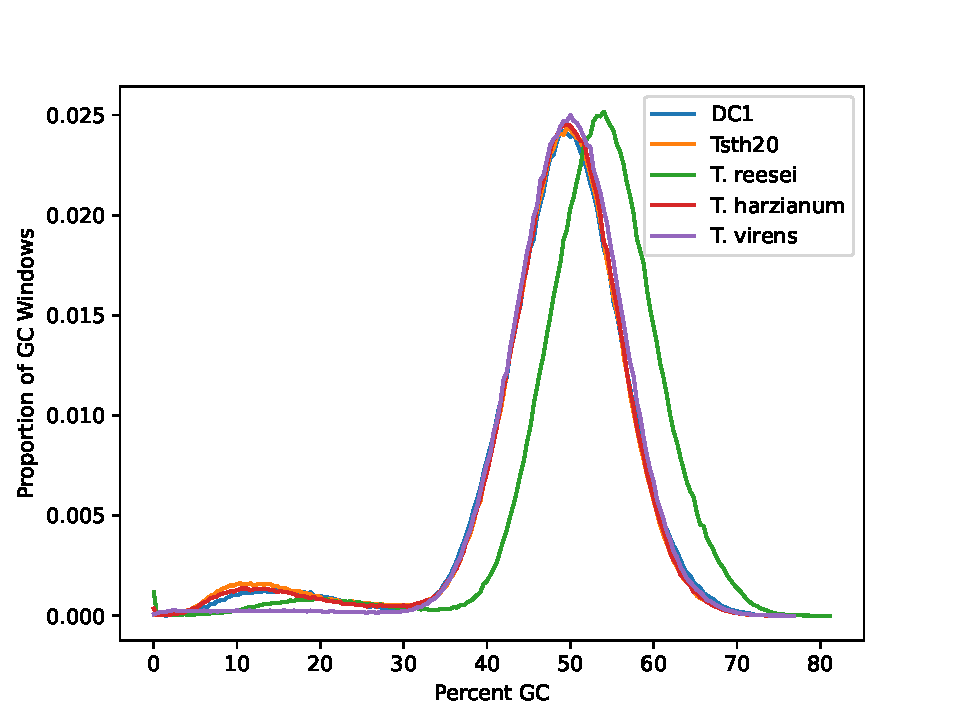
\includegraphics[width=0.8\textwidth]{figures/gc-plot.pdf}
  \end{center}
  \caption{Plots showing the frequency of GC values calculated from
    sliding windows for each assembly.}
  \label{fig:assembly-gc}
\end{figure}


